\documentclass[11pt]{beamer}
\usetheme{Boadilla}

\usepackage{agda}
\usepackage{tikz}
\usepackage{bbm}
\usepackage{animate}
\usepackage{hyperref}
\usepackage{graphicx}
\usepackage{longtable}
\usepackage{amsmath}
\usepackage{mdwlist}
\usepackage{txfonts}
\usepackage{xspace}
\usepackage{amstext}
\usepackage{amssymb}
\usepackage{stmaryrd}
\usepackage{proof}
\usepackage{multicol}
\usepackage[nodayofweek]{datetime}
\usepackage{etex}
\usepackage{textgreek}
\usepackage[all, cmtip]{xy}

\newcommand{\red}[1]{{\color{red}{#1}}}
\newcommand{\blue}[1]{{\color{blue}{#1}}}

\newenvironment{floatrule}
    {\hrule width \hsize height .33pt \vspace{.5pc}}
    {\par\addvspace{.5pc}}

\title{An Introduction to \\
Homotopy Type Theory}
\author{Amr Sabry}
\institute{
  School of Informatics and Computing \\
  Indiana University
}

\date{October 31, 2013} 

\begin{document}

\maketitle

\AgdaHide{
\begin{code}\>\<%
\\
\>\AgdaComment{-- \{-\# OPTIONS --without-K \#-\}}\<%
\\
\>\AgdaKeyword{module} \AgdaModule{talk2} \AgdaKeyword{where}\<%
\\
\>\AgdaKeyword{open} \AgdaKeyword{import} \AgdaModule{Data.Empty}\<%
\\
\>\AgdaKeyword{open} \AgdaKeyword{import} \AgdaModule{Data.Unit}\<%
\\
\>\AgdaKeyword{open} \AgdaKeyword{import} \AgdaModule{Data.Nat}\<%
\\
\>\AgdaKeyword{open} \AgdaKeyword{import} \AgdaModule{Data.Sum}\<%
\\
\>\AgdaKeyword{open} \AgdaKeyword{import} \AgdaModule{Data.Product}\<%
\\
\>\AgdaKeyword{import} \AgdaModule{Level}\<%
\\
\>\<\end{code}
}

%%%%%%%%%%%%%%%%%%%%%%%%%%%%%%%%%%%%%%%%%%%%%%%%%%%%%%%%%%%%%%%%%%%%%%%%%
\begin{frame}{Recursion and induction principles}
\vfill

Each type has a recursion and an induction principle. 

\begin{code}\>\<%
\\
\>\AgdaComment{-- for natural numbers}\<%
\\
%
\\
\>\AgdaFunction{recN} \AgdaSymbol{:} \AgdaSymbol{(}\AgdaBound{C} \AgdaSymbol{:} \AgdaPrimitiveType{Set}\AgdaSymbol{)} \AgdaSymbol{→} \AgdaBound{C} \AgdaSymbol{→} \AgdaSymbol{(}\AgdaDatatype{ℕ} \AgdaSymbol{→} \AgdaBound{C} \AgdaSymbol{→} \AgdaBound{C}\AgdaSymbol{)} \AgdaSymbol{→} \AgdaDatatype{ℕ} \AgdaSymbol{→} \AgdaBound{C}\<%
\\
\>\AgdaFunction{recN} \AgdaBound{C} \AgdaBound{c} \AgdaBound{f} \AgdaInductiveConstructor{0} \<[20]%
\>[20]\AgdaSymbol{=} \AgdaBound{c}\<%
\\
\>\AgdaFunction{recN} \AgdaBound{C} \AgdaBound{c} \AgdaBound{f} \AgdaSymbol{(}\AgdaInductiveConstructor{suc} \AgdaBound{n}\AgdaSymbol{)} \<[20]%
\>[20]\AgdaSymbol{=} \AgdaBound{f} \AgdaBound{n} \AgdaSymbol{(}\AgdaFunction{recN} \AgdaBound{C} \AgdaBound{c} \AgdaBound{f} \AgdaBound{n}\AgdaSymbol{)}\<%
\\
%
\\
\>\AgdaFunction{indN} \AgdaSymbol{:} \<[8]%
\>[8]\AgdaSymbol{(}\AgdaBound{C} \AgdaSymbol{:} \AgdaDatatype{ℕ} \AgdaSymbol{→} \AgdaPrimitiveType{Set}\AgdaSymbol{)} \AgdaSymbol{→} \<[24]%
\>[24]\<%
\\
\>[0]\AgdaIndent{8}{}\<[8]%
\>[8]\AgdaBound{C} \AgdaNumber{0} \AgdaSymbol{→} \AgdaSymbol{((}\AgdaBound{n'} \AgdaSymbol{:} \AgdaDatatype{ℕ}\AgdaSymbol{)} \AgdaSymbol{→} \AgdaBound{C} \AgdaBound{n'} \AgdaSymbol{→} \AgdaBound{C} \AgdaSymbol{(}\AgdaInductiveConstructor{suc} \AgdaBound{n'}\AgdaSymbol{))} \AgdaSymbol{→} \AgdaSymbol{(}\AgdaBound{n} \AgdaSymbol{:} \AgdaDatatype{ℕ}\AgdaSymbol{)} \AgdaSymbol{→} \AgdaBound{C} \AgdaBound{n}\<%
\\
\>\AgdaFunction{indN} \AgdaBound{C} \AgdaBound{c} \AgdaBound{f} \AgdaInductiveConstructor{0} \<[20]%
\>[20]\AgdaSymbol{=} \AgdaBound{c}\<%
\\
\>\AgdaFunction{indN} \AgdaBound{C} \AgdaBound{c} \AgdaBound{f} \AgdaSymbol{(}\AgdaInductiveConstructor{suc} \AgdaBound{n}\AgdaSymbol{)} \<[20]%
\>[20]\AgdaSymbol{=} \AgdaBound{f} \AgdaBound{n} \AgdaSymbol{(}\AgdaFunction{indN} \AgdaBound{C} \AgdaBound{c} \AgdaBound{f} \AgdaBound{n}\AgdaSymbol{)}\<%
\\
\>\<\end{code}

\end{frame}

%%%%%%%%%%%%%%%%%%%%%%%%%%%%%%%%%%%%%%%%%%%%%%%%%%%%%%%%%%%%%%%%%%%%%%%%%
\begin{frame}{Recursion and induction principles}
\vfill

Examples:

\AgdaHide{
\begin{code}\>\<%
\\
\>\AgdaKeyword{module} \AgdaModule{X} \AgdaKeyword{where}\<%
\\
\>[0]\AgdaIndent{2}{}\<[2]%
\>[2]\AgdaKeyword{open} \AgdaKeyword{import} \AgdaModule{Relation.Binary.PropositionalEquality}\<%
\\
\>\<\end{code}
}

\begin{code}\>\<%
\\
\>[0]\AgdaIndent{2}{}\<[2]%
\>[2]\AgdaFunction{double} \AgdaSymbol{:} \AgdaDatatype{ℕ} \AgdaSymbol{→} \AgdaDatatype{ℕ}\<%
\\
\>[0]\AgdaIndent{2}{}\<[2]%
\>[2]\AgdaFunction{double} \AgdaSymbol{=} \AgdaFunction{recN} \AgdaDatatype{ℕ} \AgdaNumber{0} \AgdaSymbol{(λ} \AgdaBound{n} \AgdaBound{r} \AgdaSymbol{→} \AgdaInductiveConstructor{suc} \AgdaSymbol{(}\AgdaInductiveConstructor{suc} \AgdaBound{r}\AgdaSymbol{))}\<%
\\
%
\\
\>[0]\AgdaIndent{2}{}\<[2]%
\>[2]\AgdaFunction{add} \AgdaSymbol{:} \AgdaDatatype{ℕ} \AgdaSymbol{→} \AgdaDatatype{ℕ} \AgdaSymbol{→} \AgdaDatatype{ℕ}\<%
\\
\>[0]\AgdaIndent{2}{}\<[2]%
\>[2]\AgdaFunction{add} \AgdaSymbol{=} \AgdaFunction{recN} \AgdaSymbol{(}\AgdaDatatype{ℕ} \AgdaSymbol{→} \AgdaDatatype{ℕ}\AgdaSymbol{)} \AgdaSymbol{(λ} \AgdaBound{n} \AgdaSymbol{→} \AgdaBound{n}\AgdaSymbol{)} \AgdaSymbol{(λ} \AgdaBound{m} \AgdaBound{g} \AgdaBound{n} \AgdaSymbol{→} \AgdaInductiveConstructor{suc} \AgdaSymbol{(}\AgdaBound{g} \AgdaBound{n}\AgdaSymbol{))}\<%
\\
%
\\
\>[0]\AgdaIndent{2}{}\<[2]%
\>[2]\AgdaFunction{assocAdd} \AgdaSymbol{:} \AgdaSymbol{(}\AgdaBound{i} \AgdaBound{j} \AgdaBound{k} \AgdaSymbol{:} \AgdaDatatype{ℕ}\AgdaSymbol{)} \AgdaSymbol{→} \AgdaFunction{add} \AgdaBound{i} \AgdaSymbol{(}\AgdaFunction{add} \AgdaBound{j} \AgdaBound{k}\AgdaSymbol{)} \AgdaDatatype{≡} \AgdaFunction{add} \AgdaSymbol{(}\AgdaFunction{add} \AgdaBound{i} \AgdaBound{j}\AgdaSymbol{)} \AgdaBound{k}\<%
\\
\>[0]\AgdaIndent{2}{}\<[2]%
\>[2]\AgdaFunction{assocAdd} \AgdaSymbol{=} \<[13]%
\>[13]\<%
\\
\>[2]\AgdaIndent{4}{}\<[4]%
\>[4]\AgdaFunction{indN} \<[9]%
\>[9]\<%
\\
\>[4]\AgdaIndent{6}{}\<[6]%
\>[6]\AgdaSymbol{(λ} \AgdaBound{i} \AgdaSymbol{→} \AgdaSymbol{(}\AgdaBound{j} \AgdaSymbol{:} \AgdaDatatype{ℕ}\AgdaSymbol{)} \AgdaSymbol{→} \AgdaSymbol{(}\AgdaBound{k} \AgdaSymbol{:} \AgdaDatatype{ℕ}\AgdaSymbol{)} \AgdaSymbol{→} \AgdaFunction{add} \AgdaBound{i} \AgdaSymbol{(}\AgdaFunction{add} \AgdaBound{j} \AgdaBound{k}\AgdaSymbol{)} \AgdaDatatype{≡} \AgdaFunction{add} \AgdaSymbol{(}\AgdaFunction{add} \AgdaBound{i} \AgdaBound{j}\AgdaSymbol{)} \AgdaBound{k}\AgdaSymbol{)}\<%
\\
\>[4]\AgdaIndent{6}{}\<[6]%
\>[6]\AgdaSymbol{(λ} \AgdaBound{j} \AgdaBound{k} \AgdaSymbol{→} \AgdaSymbol{?)}\<%
\\
\>[4]\AgdaIndent{6}{}\<[6]%
\>[6]\AgdaSymbol{(λ} \AgdaBound{i} \AgdaBound{h} \AgdaBound{j} \AgdaBound{k} \AgdaSymbol{→} \AgdaSymbol{?)}\<%
\\
\>\<\end{code}

\end{frame}

%%%%%%%%%%%%%%%%%%%%%%%%%%%%%%%%%%%%%%%%%%%%%%%%%%%%%%%%%%%%%%%%%%%%%%%%%
\begin{frame}{Propositions as types}
\vfill
\begin{itemize}
\vfill\item A proposition is a statement that is \red{susceptible} to proof

\vfill\item A proposition \blue{$P$} is modeled as a type;

\vfill\item If the proposition is true, the corresponding type is inhabited,
i.e., it is possible to provide evidence for \blue{$P$} using one of the
elements of the type \blue{$P$}; 

\vfill\item If the proposition is false, the corresponding type is empty,
i.e., it is impossible to provide evidence for \blue{$P$};

\vfill\item Dependent functions give us $\forall$; dependent pairs give us
$\exists$.

\end{itemize}
\vfill
\end{frame}

%%%%%%%%%%%%%%%%%%%%%%%%%%%%%%%%%%%%%%%%%%%%%%%%%%%%%%%%%%%%%%%%%%%%%%%%%
\begin{frame}{Propositions as types (ctd.)}

\begin{code}\>\<%
\\
\>\AgdaFunction{¬} \AgdaSymbol{:} \AgdaPrimitiveType{Set} \AgdaSymbol{→} \AgdaPrimitiveType{Set}\<%
\\
\>\AgdaFunction{¬} \AgdaBound{A} \AgdaSymbol{=} \AgdaBound{A} \AgdaSymbol{→} \AgdaDatatype{⊥}\<%
\\
%
\\
\>\AgdaFunction{taut1} \AgdaSymbol{:} \AgdaSymbol{\{}\AgdaBound{A} \AgdaBound{B} \AgdaSymbol{:} \AgdaPrimitiveType{Set}\AgdaSymbol{\}} \AgdaSymbol{→} \AgdaFunction{¬} \AgdaBound{A} \AgdaSymbol{→} \AgdaFunction{¬} \AgdaBound{B} \AgdaSymbol{→} \AgdaFunction{¬} \AgdaSymbol{(}\AgdaBound{A} \AgdaDatatype{⊎} \AgdaBound{B}\AgdaSymbol{)}\<%
\\
\>\AgdaFunction{taut1} \AgdaBound{na} \AgdaBound{nb} \AgdaSymbol{(}\AgdaInductiveConstructor{inj₁} \AgdaBound{a}\AgdaSymbol{)} \AgdaSymbol{=} \AgdaBound{na} \AgdaBound{a}\<%
\\
\>\AgdaFunction{taut1} \AgdaBound{na} \AgdaBound{nb} \AgdaSymbol{(}\AgdaInductiveConstructor{inj₂} \AgdaBound{b}\AgdaSymbol{)} \AgdaSymbol{=} \AgdaBound{nb} \AgdaBound{b}\<%
\\
%
\\
\>\AgdaFunction{taut2} \AgdaSymbol{:} \AgdaSymbol{\{}\AgdaBound{A} \AgdaSymbol{:} \AgdaPrimitiveType{Set}\AgdaSymbol{\}} \AgdaSymbol{→} \AgdaFunction{¬} \AgdaSymbol{(}\AgdaFunction{¬} \AgdaSymbol{(}\AgdaFunction{¬} \AgdaBound{A}\AgdaSymbol{))} \AgdaSymbol{→} \AgdaFunction{¬} \AgdaBound{A}\<%
\\
\>\AgdaFunction{taut2} \AgdaBound{nnna} \AgdaSymbol{=} \AgdaSymbol{λ} \AgdaBound{a} \AgdaSymbol{→} \AgdaBound{nnna} \AgdaSymbol{(λ} \AgdaBound{na} \AgdaSymbol{→} \AgdaBound{na} \AgdaBound{a}\AgdaSymbol{)}\<%
\\
%
\\
\>\AgdaFunction{taut3} \AgdaSymbol{:} \AgdaSymbol{\{}\AgdaBound{A} \AgdaSymbol{:} \AgdaPrimitiveType{Set}\AgdaSymbol{\}} \AgdaSymbol{→} \AgdaFunction{¬} \AgdaSymbol{(}\AgdaFunction{¬} \AgdaSymbol{(}\AgdaBound{A} \AgdaDatatype{⊎} \AgdaFunction{¬} \AgdaBound{A}\AgdaSymbol{))}\<%
\\
\>\AgdaFunction{taut3} \AgdaSymbol{=} \AgdaSymbol{λ} \AgdaBound{nana} \AgdaSymbol{→} \AgdaBound{nana} \AgdaSymbol{(}\AgdaInductiveConstructor{inj₂} \AgdaSymbol{(λ} \AgdaBound{a} \AgdaSymbol{→} \AgdaBound{nana} \AgdaSymbol{(}\AgdaInductiveConstructor{inj₁} \AgdaBound{a}\AgdaSymbol{)))}\<%
\\
\>\<\end{code}

\end{frame}

%%%%%%%%%%%%%%%%%%%%%%%%%%%%%%%%%%%%%%%%%%%%%%%%%%%%%%%%%%%%%%%%%%%%%%%%%
\begin{frame}{Identity types}
\vfill
\begin{itemize}

\vfill\item The question of whether two elements of a type are equal is
clearly a \red{proposition}

\vfill\item This proposition corresponds to a type:

\end{itemize}

\begin{code}\>\<%
\\
\>\AgdaKeyword{data} \AgdaDatatype{\_≡\_} \AgdaSymbol{\{}\AgdaBound{A} \AgdaSymbol{:} \AgdaPrimitiveType{Set}\AgdaSymbol{\}} \AgdaSymbol{:} \AgdaSymbol{(}\AgdaBound{a} \AgdaBound{b} \AgdaSymbol{:} \AgdaBound{A}\AgdaSymbol{)} \AgdaSymbol{→} \AgdaPrimitiveType{Set} \AgdaKeyword{where}\<%
\\
\>[0]\AgdaIndent{2}{}\<[2]%
\>[2]\AgdaInductiveConstructor{refl} \AgdaSymbol{:} \AgdaSymbol{(}\AgdaBound{a} \AgdaSymbol{:} \AgdaBound{A}\AgdaSymbol{)} \AgdaSymbol{→} \AgdaSymbol{(}\AgdaBound{a} \AgdaDatatype{≡} \AgdaBound{a}\AgdaSymbol{)}\<%
\\
%
\\
\>\AgdaFunction{i0} \AgdaSymbol{:} \AgdaNumber{3} \AgdaDatatype{≡} \AgdaNumber{3}\<%
\\
\>\AgdaFunction{i0} \AgdaSymbol{=} \AgdaInductiveConstructor{refl} \AgdaNumber{3}\<%
\\
%
\\
\>\AgdaFunction{i1} \AgdaSymbol{:} \AgdaSymbol{(}\AgdaNumber{1} \AgdaPrimitive{+} \AgdaNumber{2}\AgdaSymbol{)} \AgdaDatatype{≡} \AgdaSymbol{(}\AgdaNumber{3} \AgdaPrimitive{*} \AgdaNumber{1}\AgdaSymbol{)}\<%
\\
\>\AgdaFunction{i1} \AgdaSymbol{=} \AgdaInductiveConstructor{refl} \AgdaNumber{3}\<%
\\
\>\<\end{code}


\end{frame}

%%%%%%%%%%%%%%%%%%%%%%%%%%%%%%%%%%%%%%%%%%%%%%%%%%%%%%%%%%%%%%%%%%%%%%%%%
\begin{frame}{Identity types and paths}
\begin{itemize}
\vfill\item We will interpret $x ≡ y$ as a \red{path} from $x$ to $y$
\vfill\item If $x$ and $y$ are themselves paths, then $x ≡ y$ as a \red{path
between paths}, i.e., a homotopy
\vfill\item We can continue this game to get paths between paths between
paths between paths etc.
\vfill\item What are the recursion and induction principle for these paths?
\end{itemize}

\begin{code}\>\<%
\\
\>\AgdaComment{-- recursion principle}\<%
\\
\>\AgdaFunction{indiscernability} \AgdaSymbol{:} \AgdaSymbol{\{}\AgdaBound{A} \AgdaSymbol{:} \AgdaPrimitiveType{Set}\AgdaSymbol{\}} \AgdaSymbol{\{}\AgdaBound{C} \AgdaSymbol{:} \AgdaBound{A} \AgdaSymbol{→} \AgdaPrimitiveType{Set}\AgdaSymbol{\}} \AgdaSymbol{\{}\AgdaBound{x} \AgdaBound{y} \AgdaSymbol{:} \AgdaBound{A}\AgdaSymbol{\}} \AgdaSymbol{→} \<[55]%
\>[55]\<%
\\
\>[0]\AgdaIndent{2}{}\<[2]%
\>[2]\AgdaSymbol{(}\AgdaBound{p} \AgdaSymbol{:} \AgdaBound{x} \AgdaDatatype{≡} \AgdaBound{y}\AgdaSymbol{)} \AgdaSymbol{→} \AgdaBound{C} \AgdaBound{x} \AgdaSymbol{→} \AgdaBound{C} \AgdaBound{y}\<%
\\
\>\AgdaFunction{indiscernability} \AgdaSymbol{(}\AgdaInductiveConstructor{refl} \AgdaBound{x}\AgdaSymbol{)} \AgdaBound{c} \AgdaSymbol{=} \AgdaBound{c}\<%
\\
\>\<\end{code}

\end{frame}

%%%%%%%%%%%%%%%%%%%%%%%%%%%%%%%%%%%%%%%%%%%%%%%%%%%%%%%%%%%%%%%%%%%%%%%%%
\begin{frame}{K vs. J}

Bad version:

\begin{code}\>\<%
\\
\>\AgdaFunction{K} \AgdaSymbol{:} \AgdaSymbol{\{}\AgdaBound{A} \AgdaSymbol{:} \AgdaPrimitiveType{Set}\AgdaSymbol{\}} \AgdaSymbol{(}\AgdaBound{C} \AgdaSymbol{:} \AgdaSymbol{\{}\AgdaBound{x} \AgdaSymbol{:} \AgdaBound{A}\AgdaSymbol{\}} \AgdaSymbol{→} \AgdaBound{x} \AgdaDatatype{≡} \AgdaBound{x} \AgdaSymbol{→} \AgdaPrimitiveType{Set}\AgdaSymbol{)} \AgdaSymbol{→}\<%
\\
\>[2]\AgdaIndent{4}{}\<[4]%
\>[4]\AgdaSymbol{(∀} \AgdaBound{x} \AgdaSymbol{→} \AgdaBound{C} \AgdaSymbol{(}\AgdaInductiveConstructor{refl} \AgdaBound{x}\AgdaSymbol{))} \AgdaSymbol{→}\<%
\\
\>[2]\AgdaIndent{4}{}\<[4]%
\>[4]\AgdaSymbol{∀} \AgdaSymbol{\{}\AgdaBound{x}\AgdaSymbol{\}} \AgdaSymbol{(}\AgdaBound{p} \AgdaSymbol{:} \AgdaBound{x} \AgdaDatatype{≡} \AgdaBound{x}\AgdaSymbol{)} \AgdaSymbol{→} \AgdaBound{C} \AgdaBound{p}\<%
\\
\>\AgdaFunction{K} \AgdaBound{C} \AgdaBound{c} \AgdaSymbol{(}\AgdaInductiveConstructor{refl} \AgdaBound{x}\AgdaSymbol{)} \AgdaSymbol{=} \AgdaBound{c} \AgdaBound{x}\<%
\\
%
\\
\>\AgdaFunction{proof-irrelevance} \AgdaSymbol{:} \AgdaSymbol{\{}\AgdaBound{A} \AgdaSymbol{:} \AgdaPrimitiveType{Set}\AgdaSymbol{\}} \AgdaSymbol{\{}\AgdaBound{x} \AgdaBound{y} \AgdaSymbol{:} \AgdaBound{A}\AgdaSymbol{\}} \AgdaSymbol{(}\AgdaBound{p} \AgdaBound{q} \AgdaSymbol{:} \AgdaBound{x} \AgdaDatatype{≡} \AgdaBound{y}\AgdaSymbol{)} \AgdaSymbol{→} \<[57]%
\>[57]\AgdaBound{p} \AgdaDatatype{≡} \AgdaBound{q}\<%
\\
\>\AgdaFunction{proof-irrelevance} \AgdaSymbol{(}\AgdaInductiveConstructor{refl} \AgdaBound{x}\AgdaSymbol{)} \AgdaSymbol{(}\AgdaInductiveConstructor{refl} \AgdaSymbol{.}\AgdaBound{x}\AgdaSymbol{)} \AgdaSymbol{=} \AgdaInductiveConstructor{refl} \AgdaSymbol{(}\AgdaInductiveConstructor{refl} \AgdaBound{x}\AgdaSymbol{)}\<%
\\
\>\<\end{code}

\end{frame}

%%%%%%%%%%%%%%%%%%%%%%%%%%%%%%%%%%%%%%%%%%%%%%%%%%%%%%%%%%%%%%%%%%%%%%%%%
\begin{frame}{Path induction}

Good version (goes back to Leibniz)

\begin{code}\>\<%
\\
\>\AgdaComment{-- J}\<%
\\
\>\AgdaFunction{pathInd} \AgdaSymbol{:} \AgdaSymbol{\{}\AgdaBound{A} \AgdaSymbol{:} \AgdaPrimitiveType{Set}\AgdaSymbol{\}} \AgdaSymbol{→} \AgdaSymbol{(}\AgdaBound{C} \AgdaSymbol{:} \AgdaSymbol{\{}\AgdaBound{x} \AgdaBound{y} \AgdaSymbol{:} \AgdaBound{A}\AgdaSymbol{\}} \AgdaSymbol{→} \AgdaBound{x} \AgdaDatatype{≡} \AgdaBound{y} \AgdaSymbol{→} \AgdaPrimitiveType{Set}\AgdaSymbol{)} \AgdaSymbol{→} \<[54]%
\>[54]\<%
\\
\>[4]\AgdaIndent{10}{}\<[10]%
\>[10]\AgdaSymbol{(}\AgdaBound{c} \AgdaSymbol{:} \AgdaSymbol{(}\AgdaBound{x} \AgdaSymbol{:} \AgdaBound{A}\AgdaSymbol{)} \AgdaSymbol{→} \AgdaBound{C} \AgdaSymbol{(}\AgdaInductiveConstructor{refl} \AgdaBound{x}\AgdaSymbol{))} \AgdaSymbol{→} \<[39]%
\>[39]\<%
\\
\>[4]\AgdaIndent{10}{}\<[10]%
\>[10]\AgdaSymbol{(\{}\AgdaBound{x} \AgdaBound{y} \AgdaSymbol{:} \AgdaBound{A}\AgdaSymbol{\}} \AgdaSymbol{(}\AgdaBound{p} \AgdaSymbol{:} \AgdaBound{x} \AgdaDatatype{≡} \AgdaBound{y}\AgdaSymbol{)} \AgdaSymbol{→} \AgdaBound{C} \AgdaBound{p}\AgdaSymbol{)}\<%
\\
\>\AgdaFunction{pathInd} \AgdaBound{C} \AgdaBound{c} \AgdaSymbol{(}\AgdaInductiveConstructor{refl} \AgdaBound{x}\AgdaSymbol{)} \AgdaSymbol{=} \AgdaBound{c} \AgdaBound{x}\<%
\\
%
\\
\>\AgdaComment{-- for comparison}\<%
\\
\>\AgdaFunction{K'} \AgdaSymbol{:} \AgdaSymbol{\{}\AgdaBound{A} \AgdaSymbol{:} \AgdaPrimitiveType{Set}\AgdaSymbol{\}} \AgdaSymbol{(}\AgdaBound{C} \AgdaSymbol{:} \AgdaSymbol{\{}\AgdaBound{x} \AgdaSymbol{:} \AgdaBound{A}\AgdaSymbol{\}} \AgdaSymbol{→} \AgdaBound{x} \AgdaDatatype{≡} \AgdaBound{x} \AgdaSymbol{→} \AgdaPrimitiveType{Set}\AgdaSymbol{)} \AgdaSymbol{→}\<%
\\
\>[1]\AgdaIndent{5}{}\<[5]%
\>[5]\AgdaSymbol{(∀} \AgdaBound{x} \AgdaSymbol{→} \AgdaBound{C} \AgdaSymbol{(}\AgdaInductiveConstructor{refl} \AgdaBound{x}\AgdaSymbol{))} \AgdaSymbol{→}\<%
\\
\>[0]\AgdaIndent{5}{}\<[5]%
\>[5]\AgdaSymbol{∀} \AgdaSymbol{\{}\AgdaBound{x}\AgdaSymbol{\}} \AgdaSymbol{(}\AgdaBound{p} \AgdaSymbol{:} \AgdaBound{x} \AgdaDatatype{≡} \AgdaBound{x}\AgdaSymbol{)} \AgdaSymbol{→} \AgdaBound{C} \AgdaBound{p}\<%
\\
\>\AgdaFunction{K'} \AgdaBound{C} \AgdaBound{c} \AgdaSymbol{(}\AgdaInductiveConstructor{refl} \AgdaBound{x}\AgdaSymbol{)} \AgdaSymbol{=} \AgdaBound{c} \AgdaBound{x}\<%
\\
\>\<\end{code}

\end{frame}

%%%%%%%%%%%%%%%%%%%%%%%%%%%%%%%%%%%%%%%%%%%%%%%%%%%%%%%%%%%%%%%%%%%%%%%%%
\begin{frame}{Intensionality}
\begin{itemize}
\vfill\item If two terms $x$ and $y$ are \red{definitionally equal}, 
  then $x \equiv y$
\vfill\item The converse is \red{not true}
\vfill\item This gives rise to a structure of great combinatorial complexity
\end{itemize}
\vfill
\end{frame}

%%%%%%%%%%%%%%%%%%%%%%%%%%%%%%%%%%%%%%%%%%%%%%%%%%%%%%%%%%%%%%%%%%%%%%%%%
\begin{frame}{Homotopy Type Theory}
\vfill
\begin{itemize}
\vfill\item Martin-L\"of type theory
\vfill\item Identity types with path induction
\vfill\item \red{Univalence}
\vfill\item \red{Higher-Order Inductive Types}
\end{itemize}
\vfill
\end{frame}

%%%%%%%%%%%%%%%%%%%%%%%%%%%%%%%%%%%%%%%%%%%%%%%%%%%%%%%%%%%%%%%%%%%%%%%%%
\begin{frame}{Types as spaces or groupoids}

We are used to think of types as sets of values. So we think of the type Bool
as:

\begin{center}
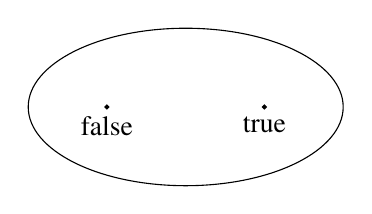
\begin{tikzpicture}
  \draw (0,0) ellipse (2cm and 1cm);
  \draw[fill] (-1,0) circle [radius=0.025];
  \node[below] at (-1,0) {false};
  \draw[fill] (1,0) circle [radius=0.025];
  \node[below] at (1,0) {true};
\end{tikzpicture}
\end{center}

In HoTT, we should instead think about it as:

\begin{center}
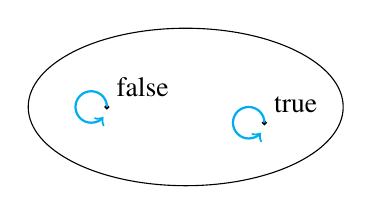
\begin{tikzpicture}
  \draw (0,0) ellipse (2cm and 1cm);
  \draw[fill] (-1,0) circle [radius=0.025];
  \draw[->,thick,cyan] (-1,0) arc [radius=0.2, start angle=0, end angle=320];
  \node[above right] at (-1,0) {false};
  \draw[fill] (1,-0.2) circle [radius=0.025];
  \draw[->,thick,cyan] (1,-0.2) arc [radius=0.2, start angle=0, end angle=320];
  \node[above right] at (1,-0.2) {true};
\end{tikzpicture}
\end{center}

\end{frame}

%%%%%%%%%%%%%%%%%%%%%%%%%%%%%%%%%%%%%%%%%%%%%%%%%%%%%%%%%%%%%%%%%%%%%%%%%
\begin{frame}{Types as spaces or groupoids}

In this particular case, it makes no difference, but in general we might have
something like:

\begin{center}
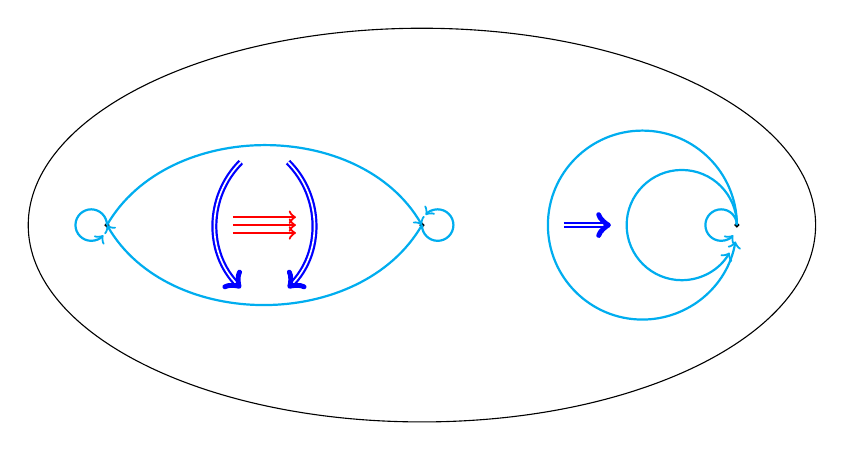
\begin{tikzpicture}
  \draw (0,0) ellipse (5cm and 2.5cm);
  \draw[fill] (-4,0) circle [radius=0.025];
  \draw[->,thick,cyan] (-4,0) arc [radius=0.2, start angle=0, end angle=320];
  \draw[fill] (0,0) circle [radius=0.025];
  \draw[->,thick,cyan] (0,0) arc [radius=0.2, start angle=-180, end angle=140];
  \draw[fill] (4,0) circle [radius=0.025];
  \draw[->,double,thick,blue] (-2.3,0.8) to [out=225, in=135] (-2.3,-0.8);
  \draw[->,double,thick,blue] (-1.7,0.8) to [out=-45, in=45] (-1.7,-0.8);
  \draw[->,thick,red] (-2.4,0.1) -- (-1.6,0.1);
  \draw[->,thick,red] (-2.4,0) -- (-1.6,0);
  \draw[->,thick,red] (-2.4,-0.1) -- (-1.6,-0.1);
  \draw[->,thick,cyan] (-4,0) to [out=60, in=120] (0,0);
  \draw[->,thick,cyan] (0,0) to [out=-120, in=-60] (-4,0);
  \draw[->,thick,cyan] (4,0) arc [radius=0.2, start angle=0, end angle=320];
  \draw[->,thick,cyan] (4,0) arc [radius=0.7, start angle=0, end angle=330];
  \draw[->,thick,cyan] (4,0) arc [radius=1.2, start angle=0, end angle=350];
  \draw[->,double,thick,blue] (1.8,0) -- (2.4,0);
\end{tikzpicture}
\end{center}

\end{frame}

%%%%%%%%%%%%%%%%%%%%%%%%%%%%%%%%%%%%%%%%%%%%%%%%%%%%%%%%%%%%%%%%%%%%%%%%%
\begin{frame}{Additional structure}
\begin{itemize}

\vfill\item For every path $p : x \equiv y$, there exists a path $! p : y
\equiv x$;

\vfill\item For every paths $p : x \equiv y$ and $q : y \equiv z$, there
exists a path $p \circ q : x \equiv z$;

\vfill\item Subject to the following conditions:
  \begin{itemize}
  \vfill\item $p \circ \mathit{refl}~y \equiv p$
  \vfill\item $p \equiv \mathit{refl}~x \circ p$
  \vfill\item $!p \circ p \equiv \mathit{refl}~y$
  \vfill\item $p ~\circ~ !p \equiv \mathit{refl}~x$
  \vfill\item $!~(!p) \equiv p$
  \vfill\item $p \circ (q \circ r) \equiv (p \circ q) \circ r$
  \end{itemize}

\vfill\item With similar conditions one level up and so on and so forth.

\end{itemize}
\vfill
\end{frame}

%%%%%%%%%%%%%%%%%%%%%%%%%%%%%%%%%%%%%%%%%%%%%%%%%%%%%%%%%%%%%%%%%%%%%%%%%
\begin{frame}{Pause}

\vfill
\begin{center}
\LaTeX\ crash \ldots \\
Switch to third talk
\end{center}
\vfill

\end{frame}

%%%%%%%%%%%%%%%%%%%%%%%%%%%%%%%%%%%%%%%%%%%%%%%%%%%%%%%%%%%%%%%%%%%%%%%%%
\end{document}

%%%%%%%%%%%%%%%%%%%%%%%%%%%%%%%%%%%%%%%%%%%%%%%%%%%%%%%%%%%%%%%%%%%%%%%%%
\begin{frame}{}
\vfill
\begin{itemize}
\vfill\item
\vfill\item
\vfill\item
\end{itemize}
\vfill
\end{frame}

%%%%%%%%%%%%%%%%%%%%%%%%%%%%%%%%%%%%%%%%%%%%%%%%%%%%%%%%%%%%%%%%%%%%%%%%%
\begin{frame}{}

\begin{code}\>\<%
\\
%
\\
\>\<\end{code}

\end{frame}

